% !TEX encoding = UTF-8
% !TEX TS-program = pdflatex
% !TEX root = ../tesi.tex
% !TEX spellcheck = it-IT

%**************************************************************
\chapter{Valutazione retrospettiva}
\label{cap:valutazione-retrospettiva}
%**************************************************************

\intro{Questo capitolo contiene un resoconto sull'intera attività di stage}\\

\section{Resoconto sugli obiettivi produttivi}

L'attività di stage aveva come scopo, per l'azienda, lo sviluppo di diverse
funzionalità per JPA che andassero ad estendere le possibilità che
l'applicazione offriva prima del mio arrivo.

Ad inizio stage, ho definito con il tutor aziendale gli obiettivi presenti in
tabella \ref{tab:obiettivi-produttivi}. In tabella
\ref{tab:obiettivi-produttivi-realizzati} è presente l'esito relativo al
raggiungimento di questi. \\

{
\centering
\begin{tabular}{| p{8cm} | c |}

\hline
\textbf{Obiettivo definito} & \textbf{Risultato} \\
\hline
Confronto tra stato attuale di JPA e Scrum ``puro'' &
Realizzato \\
\hline
Sviluppo di un modulo di checklist &
Realizzato \\
\hline
Sviluppo di una \gloss{direttiva} per visualizzare un burn-down chart per uno
  sprint &
Realizzato \\
\hline
Avvio di un'istanza di processo da un task &
Realizzato \\
\hline
Sviluppo di un sistema di notifiche push &
Realizzato \\
\hline
Collegamento tra area Scrum e Forum &
Realizzato \\
\hline
\end{tabular}
\captionof{table}{Obiettivi produttivi realizzati}
\label{tab:obiettivi-produttivi-realizzati}
}
\rule{0pt}{2ex}

Oltre a quelli esposti in tabella \ref{tab:obiettivi-produttivi-realizzati},
sono stati individuati ulteriori sviluppi ad attività in corso, dal momento
che il lavoro complessivo previsto è stato svolto anticipatamente e che la
gestione degli obiettivi è stata particolarmente flessibile (cfr. sez.
\ref{sec:visione-gestione-ob}).

Per questo motivo, alcuni obiettivi sono stati stabiliti ed alcuni di quelli
già presenti sono stati estesi. \\

{
\centering
\begin{tabular}{| p{6cm} | p{6cm} |}

\hline
\textbf{Obiettivo esteso} & \textbf{Obiettivo aggiuntivo} \\
\hline
Sviluppo di una \gloss{direttiva} per visualizzare un burn-down chart per uno
  sprint &
Sviluppo di strumenti di \emph{Inspection} e relativo modulo \\
\hline
Sviluppo di un sistema di notifiche push &
Sviluppo di notifiche via Telegram (inizialmente erano previste solamente le
  notifiche via mail interna) \\
\hline
Sviluppo di notifiche via Telegram &
Prototipazione di servizi generici con Telegram Bot \\
\hline
\end{tabular}
\captionof{table}{Obiettivi produttivi aggiuntivi}
\label{tab:obiettivi-produttivi-aggiunti}
}
\rule{0pt}{2ex}

Le aggiunte presenti in tabella \ref{tab:obiettivi-produttivi-aggiunti}
derivano anche da stime errate compiute durante l'attività di pianificazione.
Tale errore è amplificato dal fatto che il 60\% del tempo dell'ultima
settimana è stato impiegato per conoscere più approfonditamente la realtà
aziendale descritta nel primo capitolo del presente documento.

Personalmente, ritengo che il lavoro aggiuntivo avrebbe potuto essere previsto
anticipatamente per i seguenti motivi:

\begin{itemize}
\item Sebbene non avessi mai sviluppato software avvalendomi dei
  \gloss{framework} utilizzati nell'attività di stage, conoscevo le tecnologie
  alla base di questi;
\item In alcuni corsi di laurea erano state fornite delle basi per la
  comprensione dei \gloss{framework} a me nuovi;
\item Una volta sviluppato un incremento e compreso l'architettura alla base
  di tutte le aree di JPA (sia nella parte di \FREND{} che di \BKEND{}), lo
  sforzo necessario per replicare correttamente tali componenti o applicare
  modifiche a queste è stato decisamente più contenuto.
\end{itemize}

Allo stesso tempo, io stesso ad inizio stage ritenevo che la pianificazione
effettuata fosse corretta dal momento che:

\begin{itemize}
\item Non considerando i progetti universitari, la mia esperienza in fatto di
  realizzazione o estensione di sistemi informatici era limitata;
\item Proprio per il fatto che ritenevo la mia esperienza applicativa molto
  limitata, pensavo che anche l'apprendimento di nuovi \gloss{framework}
  avrebbe impegnato maggior tempo di quanto effettivamente speso.
\end{itemize}

Un altro modo per valutare il raggiungimento di obiettivi produttivi è guardare
la copertura dei requisiti.

Con questa visione, è possibile notare che tutti gli obiettivi obbligatori sono
stati soddisfatti, mentre non tutti gli obiettivi desiderabili o opzionali
sono stati portati a termine:

\begin{itemize}
\item Come detto in fondo alla sezione \ref{sec:prog-codifica}, durante lo
  stage non erano disponibili le \gloss{api} per la ricezione e il salvataggio
  di file inviati ad un Telegram Bot (RF2.1Des relativo alla prototipazione
  per Telegram Bot, tabella \ref{tab:requisiti-prototipo});
\item Non sempre le raccomandazioni di sviluppo aziendali o adottate da me sono
  state rispettate.
\end{itemize}

Come è possibile vedere in figura \ref{fig:requisiti-soddisfacimento}, il
97,7\% dei requisiti è stato soddisfatto.

\begin{figure}[H]%
\centering
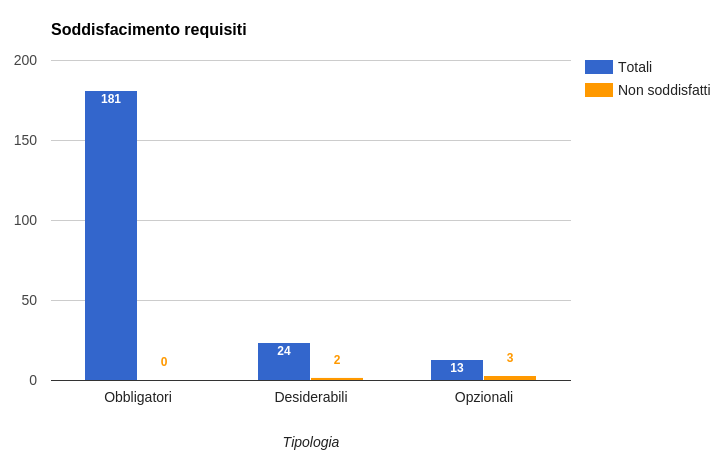
\includegraphics[width=1.1\columnwidth]{immagini/requisiti}
\caption{Soddisfacimento dei requisiti a fine stage}
\label{fig:requisiti-soddisfacimento}%
\end{figure}

\section{Resoconto sugli obiettivi formativi}

I risultati relativi agli obiettivi formativi sono stati riportati nella
tabella \ref{tab:obiettivi-formativi-realizzati}. \\

{
\centering
\begin{tabular}{| p{6cm} | p{6cm} |}

\hline
\textbf{Obiettivo previsto} & \textbf{Risultato} \\
\hline
Ottenimento di una conoscenza profonda di Scrum &
Realizzato \\
\hline
Acquisizione delle competenze necessarie per sviluppare le funzionalità
  previste negli obiettivi produttivi &
Realizzato \\
\hline
Capacità di adattare i principi di Scrum ad esigenze diverse dallo sviluppo
  software &
Parzialmente realizzato \\
\hline
\end{tabular}
\captionof{table}{Obiettivi formativi}
\label{tab:obiettivi-formativi-realizzati}
}
\rule{0pt}{2ex}

L'obiettivo riguardante l'adattamento dei principi di Scrum ad esigenze diverse
dallo sviluppo software è ritenuto parzialmente realizzato per i seguenti
motivi:

\begin{itemize}
\item In parte del tempo speso durante l'ultima settimana e durante lo studio
  della parte di modellazione processi, ho esteso la mia conoscenza riguardo
  la realtà aziendale e ho visto esempi di come Sanmarco Informatica offre il
  proprio \emph{know how} ad aziende di settori diversi dal suo (e.g. che
  adottano la \emph{lean production} e non Scrum a supporto dei propri
  processi);
\item Per ciascuno degli strumenti di \emph{Inspection} è stata valutata la
  possibilità di utilizzare questi nell'ambito dell'analisi di processi nel
  documento in cui essi erano descritti;
\item Durante lo studio della metodologia Scrum, diverse fonti contenevano
  informazioni su come i metodi agili fossero nati, di come questi si fossero
  ispirati al \textbf{TPS} (Toyota Production System) e la storia di questo;
\item Le funzionalità introdotte sono state sviluppate tenendo conto
  che queste potrebbero essere riusate per scopi diversi dall'applicazione di
  Scrum\footnote{Ad esempio, gli strumenti di \emph{Inspection} possono essere
  visti come mezzi con cui analizzare cicli produttivi di breve durata.}. Hanno
  fatto eccezione il collegamento dell'area Scrum al forum e alla parte di
  modellazione di processi, siccome erano fortemente legate a elementi
  caratteristici di Scrum;
\item Durante lo stage gli unici \emph{stakeholder} per l'area Scrum erano i
  componenti del team in cui ero inserito. Di conseguenza, non ho potuto
  verificare se effettivamente quanto ho sviluppato sia concretamente
  utilizzabile per processi di produzione di beni o servizi diversi dal
  software.
\end{itemize}

Riguardo agli obiettivi formativi riportati in tabella
\ref{tab:obiettivi-formativi-realizzati}, ho maturato riflessioni su diversi
aspetti dello stage.

\subsection{Disponibilità del team} \mbox{} \\

L'apprendimento è stato notevolmente facilitato dalla disponibilità continua
del tutor aziendale e degli altri elementi del team. Infatti ho ricevuto:

\begin{itemize}
\item Precise linee guida di sviluppo;
\item Aiuto quando ho trovato difficoltà nel procedere con il lavoro;
\item Utili consigli su come migliorare l'efficienza per l'esecuzione di
  operazioni SQL e sostegno durante le discussioni per capire quali dati
  estrarre per la creazione di burn-down chart e quale fosse il miglior modo
  per estrarli.
\end{itemize}

\subsection{Comportamento e struttura dell'applicazione Web} \mbox{} \\

Sebbene non avessi mai utilizzato HTML5 e AngularJS, partivo da una buona
conoscenza di XHTML 1.0 e Javascript ``puro''. Ciò ha influito nel seguente
modo nella mia formazione durante il periodo di stage:

\begin{itemize}
\item HTML5 è un linguaggio che deriva da XHTML. Grazie a questo fattore, mi
  è stato sufficiente individuare le differenze più importanti tra i due per
  non aver grosse difficoltà a sviluppare la parte strutturale delle pagine
  del \FREND;
\item AngularJS è sensibilmente diverso da Javascript. Tuttavia, grazie
  a quanto imparato nel modulo B del corso di Ingegneria del Software, alla
  letteratura utilizzata e alla documentazione trovata su Internet, ho potuto
  far mie alcune delle notevoli possibilità offerte da questo
  \gloss{framework}.
\end{itemize}

\subsection{Architettura del \FREND{}} \mbox{} \\

Prima dell'attività di stage, non avevo mai sviluppato un'applicazione Web che
fosse contenuta interamente in una sola pagina. Tuttavia, prima dello stage ho
investito parte del mio tempo vedendo come le \gloss{spa} potessero essere
realizzate con AngularJS e le conseguenze che ciò comportava.

In questo modo, ottenere una visione d'insieme dei vari moduli contenuti in
JPA è stato più facile una volta iniziato lo stage.

\subsection{Componente presentazionale di pagine Web} \mbox{} \\

L'uso di TODC Bootstrap ha semplificato di molto lo sviluppo della parte di
presentazione delle pagine siccome, tramite l'uso di tag o di attributi di
carattere semantico durante la realizzazione della struttura, tale
\gloss{framework} riusciva a fornire lo stile adatto ai vari elementi della
pagina.

\subsection{Gestione delle chiamate \gloss{rest}} \mbox{} \\

Le \gloss{jaxrs} erano a me nuove e per la gestione di chiamate \gloss{rest}
non avevo mai utilizzato Java finora.

Tuttavia, la semplicità delle \gloss{jaxrs} mi ha permesso di capire in poche
ore come poterle utilizzare e come generare le classi della \emph{business
logic} per ricevere dati con chiamate \gloss{rest} provenienti dal \FREND.

\subsection{Utilizzo di SQL} \mbox{} \\

Per l'interazione con i \gloss{rdbms} era previsto l'uso di comandi SQL
(linguaggio a me noto già da prima dell'attività di stage) tramite il package
\texttt{java.sql}. Anche se non avevo mai realizzato programmi che facessero
uso di questo package, il suo uso si è rivelato semplice ed intuitivo.

\subsection{Scrum} \mbox{} \\

Prima dello stage, Scrum e metodi agili per me erano solamente interessanti
campi di studio, poichè non avevo mai avuto modo di poterli vivere sulla mia
pelle come metodologie di lavoro.

Grazie all'attività di stage, ho potuto:

\begin{itemize}
\item Capire meglio quali esigenze e quali motivazioni hanno portato le aziende
  ad adottare Scrum;
\item Sperimentare una realtà in cui Scrum veniva usato quotidianamente;
\item Capire quali benefici derivano dall'applicazione di questo metodo;
\item Scoprire delle interessanti attività di supporto a Scrum come il
  \textbf{Planning
  Poker}\footnote{\url{https://en.wikipedia.org/wiki/Planning_poker}};
\item Studiare anche i possibili effetti negativi che potrebbero derivare da
  una scorretta applicazione di questo e le cause principali di questi.
\end{itemize}

\section{Distanza tra corso di studi e realtà aziendale}

Ad inizio stage non sapevo precisamente quanto di quello che ho visto in ateneo
avrei trovato in una realtà aziendale.

Ad attività finità, ho maturato le seguenti considerazioni:

\subsection{Verifica dinamica}

In alcuni insegnamenti universitari viene posta particolare enfasi nel
progettare test per i propri programmi.
Questa attività serve infatti per ridurre la verifica manuale sia da parte di
sviluppatori che di verificatori.

Oltre a notevoli risparmi in termini di tempo e denaro durante lo sviluppo, i
test automatici portano grandi risparmi quando si tratta di svolgere
manutenzione: cambiando una parte di un programma, è sempre necessario
verificare che tutto il resto funzioni ancora e, nel caso in cui questo
controllo venga eseguito manualmente, ciò costituisce un'intera ripetizione del
ciclo di verifica dinamica.

Tuttavia, nella realtà industriale che ho conosciuto questa pratica non è
diffusa anche se il suo impiego avrebbe probabilmente comportato guadagni per
l'azienda.

\subsection{UML}

Nel'insegnamento di Ingegneria del Software vengono visti diversi tipi di
diagramma \gloss{uml} per vari scopi: definizione degli scenari possibili di un
programma, analisi della sua esecuzione, analisi della sua architettura o
dell'interazione fra componenti, etc.

Per quanto ho potuto vedere, a livello industriale non tutti gli strumenti
tecnologici visti nel mondo accademico sono presenti o utilizzati, ad esempio
spesso è preferita la realizzazione di mockup o spiegazioni di tipo discorsivo
sul lavoro che bisogna svolgere.

Nel caso del mio stage, l'introduzione di strumenti come i diagrammi
\gloss{uml} ha permesso di esprimere più chiaramente alcuni concetti discussi
con gli \emph{stakeholder}, rimuovendo ambiguità e fornendo di fatto uno
strumento efficace per il dialogo.

\subsection{Design pattern}

All'interno di JPA non ho notato l'uso di \gloss{design-pattern}, a meno che
questi non siano direttamente imposti o implementati nativamente dai
\gloss{framework} utilizzati.

Per quanto ho potuto vedere, ad esempio nel progetto di Ingegneria del
Software, i \gloss{design-pattern} costituiscono invece una componente
fondamentale per architetture di sistemi informatici, poichè garantiscono
molte qualità ed evitano di incorrere nei cosidetti \emph{anti-pattern}, come
ad esempio il già menzionato \gloss{telescoping}.

\subsection{Strumenti e procedure per la qualità}

In tutti gli insegnamenti universitari in cui fosse previsto un progetto o la
realizzazione di un programma per il superamento dell'esame, ho notato che
veniva riposta particolare attenzione su delle qualità specifiche per ogni
materia di studio.

Durante l'attività di stage non ho invece notato particolari strumenti che
imponessero il rispetto di standard di tipo qualitativo, se non le norme e
raccomandazioni adottate dal team di sviluppo.

A causa di ciò, ho semplicemente cercato di perseguire le qualità viste
all'Università affinchè architettura e codice fossero facilmente estendibili e
comprensibili:

\begin{itemize}
\item Uso di pre-condizioni, post-condizioni e invariante nei frammenti di
  codice più complessi;
\item Uso di Javadoc;
\item Uso di \gloss{design-pattern} architetturali;
\item Contenimento della complessità ciclomatica e del numero dei livelli di
  annidamento;
\item Limitare la lunghezza dei metodi e il numero di parametri per metodo;
\item Incapsulazione -- la maggior parte delle classi pre-esistenti aveva i
  campi dati degli oggetti ad accesso pubblico, mentre per le classi di
  package di mia creazione ho ristretto l'accesso a tali membri delle entità.
\end{itemize}

\subsection{Tecnologie emergenti}

A differenza di molte startup o aziende consolidate, durante la mia esperienza
all'Università ho avuto raramente a che fare con tecnologie emergenti o
innovative.

Molti insegnamenti infatti si basano su tecnologie consolidate e stabili e,
sebbene siano usate frequentemente dalle aziende, ciò comporta che sia per
progetti didattici che per lo svolgimento di esami si impieghino solamente
quelle.

Se da un lato può costituire senza dubbio una garanzia in termini di
prospettiva occupazionale, dall'altro è vero che quando ho affrontato lo stage
mi trovavo per la prima volta ad utilizzare tecnologie attualmente diffuse
come AngularJS o Bootstrap\footnote{Al momento della stesura della tesi, il
\gloss{framework} originale (non quello proposto da TODC) è il progetto con
più preferenze, ovvero 86583 utenti, su GitHub.}.

Un altro esempio possono essere Python e Ruby on Rails: questi linguaggi,
comunemente diffusi a livello industriale, non vengono mai mostrati in alcun
corso (se non incidentalmente in alcuni progetti di Ingegneria del Software).

\subsection{Importanza degli insegnamenti}

Il fatto di aver completato anticipatamente gli obiettivi mi ha fatto capire
ancor di più quanto l'Università prepari i propri studenti non tanto a
specializzarsi per essere uno sviluppatore di un certo linguaggio, ma ad
essere una figura professionale in grado di adattarsi e avente conoscenze tali
da poter affrontare problemi con molta più facilità rispetto a persone che non
hanno seguito questo percorso.

Ritengo infatti che i seguenti corsi abbiano contribuito significativamente
alla buona riuscita dello stage:

\begin{itemize}
\item \textbf{Ingegneria del software:} questo insegnamento e il relativo
  progetto mi hanno permesso di acquisire delle conoscenze e competenze che si
  sono rivelate molto utili, tra cui:
  \begin{itemize}
  \item Conoscenza di Scrum e confronto di questa metodologia con altri modelli
    di sviluppo software;
  \item Uso di sistemi di versionamento e l'analisi sulle varie modalità di
    impiego di questi;
  \item Conoscenza di qualità da ricercare per architetture e codice sorgente;
  \item Capacità di produrre documenti di natura uniforme tra loro e riuso
    sistematico di documenti sviluppati precedentemente;
  \item Conoscenza ed uso dei diagrammi \gloss{uml};
  \item Individuazione di norme e raccomandazioni a supporto dei processi di
    sviluppo;
  \item \Gloss{best-practice} per le attività di analisi e progettazione;
  \item Uso dei \gloss{design-pattern}.
  \end{itemize}
\item \textbf{Programmazione e Algoritmi e Strutture Dati:} le abilità
  acquisite in questi insegnamenti mi hanno permesso di affrontare facilmente
  le complessità algoritmiche dovute a:
  \begin{itemize}
  \item Preparare i dati per i burn-down chart: era necessario un algoritmo che
    fosse efficiente e capace di soddisfare tutti i requisiti imposti;
  \item Realizzazione del linguaggio per le notifiche: questo problema è stato
    affrontato con raffinamenti successivi di uno dei semplici algoritmi di
    ricerca di occorrenze in un testo visti nel corso di Programmazione.
  \end{itemize}
\item \textbf{Programmazione ad oggetti:} questo insegnamento mi ha permesso
  di capire a fondo i principi cardine della programmazione ad oggetti;
\item \textbf{Programmazione concorrente e distribuita:} con questo
  insegnamento ho appreso le \gloss{best-practice} e le caratteristiche più
  importanti di Java, linguaggio largamente usato durante l'attività di stage;
\item \textbf{Data Mining:} le conoscenze acquisite in questo insegnamento,
  inserito a libera scelta nel piano di studi, mi hanno aiutato principalmente
  in due occasioni:
  \begin{itemize}
  \item Realizzazione della curva di carico ``reale'' nei burn-down chart;
  \item Analisi critica dei dati presenti nei vari strumenti di
    \emph{Inspection} e capacità di descrivere cosa si può ricavare da questi.
  \end{itemize}
\item \textbf{Tecnologie Web:} insegnamento in cui viene posta molta attenzione
  sull'accessibilità dei siti Web e sulla buona realizzazione di struttura e
  presentazione di questi, mi ha aiutato ad essere pronto per imparare ad
  usare i vari \gloss{framework} per il \FREND;
\item \textbf{Basi di dati:} dal momento che durante lo stage ho dovuto
  progettare tabelle e realizzare delle interrogazioni per ricavare dati da
  queste, l'insegnamento mi ha fornito le giuste basi teoriche e pratiche per
  poter effettuare entrambe le attività.
\end{itemize}

\subsection{Collaborazione studenti-professori}

A differenza di altre Università, nel Corso di Laurea triennale vi sono poche
inziative che coinvolgono attivamente studenti e professori.

Questo aspetto è a mio parere limitante per le possibilità che l'Università
degli Studi di Padova potrebbe offrire, visto che attività del genere
potrebbero fornire sia dell'utile \emph{know-how} come preparazione per il
mondo del lavoro che interessanti spunti su svariati campi di ricerca.

\subsection{Progetti didattici}

Alcuni progetti durante il corso di studi sono di tipo \emph{one-off}, mentre
altri riescono a fornire conoscenze e competenze che sono riutilizzabili in un
secondo momento.

Questo non è dovuto a mio parere alla qualità degli insegnamenti, ma al peso e
al tempo dedicato per tali progetti. Per questo motivo, alcuni progetti di
taglia minore potrebbero essere uniti per realizzare una base solida di abilità
da poter utilizzare nel mondo del lavoro.
